\documentclass{article}
\usepackage[utf8]{inputenc}
\usepackage[english]{babel}
\usepackage[]{amsthm} %lets us use \begin{proof}
\usepackage[]{amssymb} %gives us the character \varnothing
\usepackage[]{setspace} %provides commands to set line spacing
\usepackage[left=0.75in, right=0.75in]{geometry}
\usepackage{hyperref}
\usepackage{xcolor}
\usepackage{amsmath}
\usepackage{enumitem}
\usepackage{graphicx}
\usepackage{subfigure}
\usepackage{float}
\usepackage{float}
\title{Homework 4}
\author{Son [Joe] Nguyen}
%\date{\today}

\begin{document}
%\maketitle %This command prints the title based on information entered above
\begin{center}
	\LARGE{Homework 4}\\[1em]
	\large Son [Joe] Nguyen\\[1em]
	%\large \today
\end{center}
\subsection*{Problem 2.19}
\[f(x) = \sum_{n=0}^{\infty} \left[a_n \sin \left(\frac{n\pi x}{a}\right) + b_n \cos \left(\frac{n \pi x}{a}\right)\right]\]
We have:
\[e^{ix} = \cos x + i\sin x \]
\[\Rightarrow e^{i\left(\frac{n \pi x}{a}\right)} = \cos \left(\frac{n \pi x}{a}\right) + i \sin \left(\frac{n \pi x}{a}\right)\]
\[\Rightarrow e^{-i\left(\frac{n \pi x}{a}\right)} = \cos \left(\frac{n \pi x}{a}\right) - i \sin \left(\frac{n \pi x}{a}\right)\]
Adding and subtracting the two equations above, we have:
\[e^{i\left(\frac{n \pi x}{a}\right)} + e^{-i\left(\frac{n \pi x}{a}\right)} = 2\cos \left(\frac{n \pi x}{a}\right)\]
\[e^{i\left(\frac{n \pi x}{a}\right)} - e^{-i\left(\frac{n \pi x}{a}\right)} = 2 i \sin \left(\frac{n \pi x}{a}\right)\]

\begin{align*}
	f(x) & = b_o + \sum_{n=1}^{\infty} \left[a_n \sin \left(\frac{n\pi x}{a}\right) + b_n \cos \left(\frac{n \pi x}{a}\right)\right]                                                                    \\
	     & = b_0 + \sum_{n=1}^{\infty} a_n \left(\frac{e^{i(\frac{n \pi x}{a})} - e^{-i \frac{n \pi x}{a}}}{2i}\right) + b_n \left(\frac{e^{i(\frac{n \pi x}{a})} + e^{-i \frac{n \pi x}{a}}}{2}\right) \\
	     & = b_0 + \sum_{n=1}^{\infty} \left(\frac{a_n}{2i} + \frac{b_n}{2}\right)e^{i(\frac{n \pi x}{a})} + \left(\frac{b_n}{2} - \frac{a_n}{2i}\right)e^{-i(\frac{n \pi x}{a})}                       \\
\end{align*}
when $n = 0$, we have \(c_0 = b_0\), when $n > 0$, we have \(c_n = \frac{-i a _n + b_n}{2}\), and when $n < 0$, we have \(c_n = \frac{i a_{-n} + b_{-n}}{2} \):
\begin{align*}
	f(x) & = c_0 + \sum_{n=1}^{\infty} c_n e^{i(\frac{n \pi x}{a})} + \sum_{n = -1 }^{-\infty} c_n e^{i(\frac{n \pi x}{a})} \\
	     & = \sum_{n = -\infty}^{\infty} c_n e^{i(\frac{n \pi x}{a})}                                                       \\
\end{align*}
Using the equation above, we have:
\[f(x) e^{\frac{- i n \pi x}{a}} = \sum_{k = -\infty}^{\infty} c_k e^\frac{i (n - k) \pi x}{a }\]  multiply both sides by \(e^{\frac{-i n \pi x}{a}}\)
\\
\\
Now we integrate both sides from \(-a\) to \(a\):
\begin{align*}
	\int_{-a}^{a} f(x) e^{\frac{- i n \pi x}{a}} dx & = \int_{-a}^{a} \sum_{k = -\infty}^{\infty} c_k e^\frac{i (n - k) \pi x}{a } dx \quad \text{now we simplify the right hand side of the equation} \\
	                                                & = \sum_{k = -\infty}^{\infty} c_k \int_{-a}^{a} e^\frac{i (n - k) \pi x}{a } dx                                                                  \\
\end{align*}
For the intergration on the right hand side, when \(k \neq n \), we have:
\begin{align*}
	\int_{-a}^{a} e^\frac{i (n - k) \pi x}{a } dx & = \frac{a}{i (n - k) \pi} \left[e^\frac{i (n - k) \pi x}{a }\right]_{-a}^{a}                                      \\
	                                              & = \frac{a}{i (n - k) \pi} \left[e^\frac{i (n - k) \pi a}{a } - e^\frac{-i (n - k) \pi a}{a }\right]               \\
	                                              & = \frac{a}{i (n - k) \pi} \left[e^{i (n - k) \pi } - e^{-i (n - k) \pi }\right]                                   \\
	                                              & = \frac{a}{i (n - k) \pi} \left(\cos((n-k) \pi) + i \sin ((n-k) \pi) - (\cos((k-n)\pi) - i \sin((k-n)\pi))\right) \\
	                                              & = 0
\end{align*}
When \(k = n\), we have:
\begin{align*}
	\int_{-a}^{a} e^\frac{i (n - k) \pi x}{a } dx & = \int_{-a}^{a} e^\frac{i (n - n) \pi x}{a } dx \\
	                                              & = \int_{-a}^{a} e^0 dx                          \\
	                                              & = \int_{-a}^{a} 1 dx                            \\
	                                              & = 2a
\end{align*}
Therefore, we have:
\begin{align*}
	\int_{-a}^{a} f(x) e^{\frac{- i n \pi x}{a}} dx & = \sum_{k = -\infty}^{\infty} c_k \int_{-a}^{a} e^\frac{i (n - k) \pi x}{a } dx \\
	                                                & = c_n \int_{-a}^{a} e^\frac{i (n - n) \pi x}{a } dx                             \\
	                                                & = c_n 2a                                                                        \\
\end{align*}
\[\Rightarrow c_n = \frac{1}{2a} \int_{-a}^{a} f(x) e^{\frac{- i n \pi x}{a}} dx\]

Substitute \(k = \frac{n \pi}{a}\) into \(f(x)\):
\begin{align*}
	f(x) & = \sum_{n = -\infty}^{\infty} c_n e^{i k_n x}                                       \\
	     & = \frac{1}{\sqrt{2 \pi}} \sum_{n = -\infty}^{\infty} (\sqrt{2 \pi} c_n) e^{i k_n x} \\
\end{align*}
Now we just need to prove that \(\sqrt{2 \pi} c_n = F(k) \Delta k\):

\begin{align*}
	\sqrt{2 \pi} c_n & = \sqrt{2 \pi} \frac{1}{2a} \int_{-a}^{a} f(x) e^{\frac{- i n \pi x}{a}} dx                         \\
	                 & = \frac{1}{\sqrt{2 \pi}} \frac{2 \pi}{2 a} \int_{-a}^{a} f(x) e^{\frac{- i n \pi x}{a}} dx          \\
	                 & = \left[\frac{1}{\sqrt{2 \pi}} \int_{-a}^{a} f(x) e^{\frac{- i n \pi x}{a}} dx\right] \frac{\pi}{a} \\
	                 & = F(k_n) \Delta k
\end{align*}
From the previous part, we have:
\[f(x) = \frac{1}{\sqrt{2 \pi}} \sum_{n = - \infty}^{\infty} F(k_n)e^{ik_n x} \Delta k \quad , k_n = \frac{n \pi}{a}\]
\[F(k_n) = \frac{1}{\sqrt{2 \pi}} \int_{-a}^{a} f(x) e^{-i k_n x} dx\]
For the function \(f(x)\), when \(a \rightarrow \infty\):
\begin{align*}
	f(x) & = \frac{1}{\sqrt{2 \pi}} \int_{-\infty}^{\infty} F(k) e^{i k x} dk  \\
	F(k) & = \frac{1}{\sqrt{2 \pi}} \int_{-\infty}^{\infty} f(x) e^{-i k x} dx
\end{align*}

\subsection*{Problem 2.20}
\[\Psi(x,0) = A e^{-a|x|}\]
\begin{enumerate}[label=(\alph*)]
	\item Normalize the wave function:
	      \begin{align*}
		      1                     & = \int_{-\infty}^{\infty} |\Psi(x,0)|^2 dx   \\
		                            & = \int_{-\infty}^{\infty} |A e^{-a|x|}|^2 dx \\
		                            & = A^2 \int_{-\infty}^{\infty} e^{-2a|x|} dx  \\
		                            & = A^2 2 \int_{0}^{\infty} e^{-2a x} dx       \\
		                            & = A^2 2 \frac{1}{2a}                         \\
		      \Rightarrow A         & = \sqrt{a}                                   \\
		      \Rightarrow \Psi(x,0) & = \sqrt{a} e^{-a|x|}
	      \end{align*}
	\item we have:
	      \[\Psi(x,t) = \frac{1}{\sqrt{2\pi}} \int_{-\infty}^{\infty} \phi(k) e^{i(kx - \omega t)}dk\]
	      \[\phi(k) = \frac{1}{\sqrt{2 \pi}} \int_{-\infty}^{\infty} \Psi(x,0) e^{-ikx} dx\]
	      \begin{align*}
		      \phi(k) & = \frac{1}{\sqrt{2 \pi}} \int_{-\infty}^{\infty} \sqrt{a} e^{-a|x|} e^{-ikx} dx                                                          \\
		              & = \frac{\sqrt{a}}{\sqrt{2 \pi}} \int_{-\infty}^{\infty} e^{-a|x|-ikx} dx                                                                 \\
		              & = \frac{\sqrt{a}}{\sqrt{2 \pi}} \int_{-\infty}^{0}  e^{-a|x|-ikx} dx + \frac{\sqrt{a}}{\sqrt{2 \pi}} \int_{0}^{\infty}  e^{-a|x|-ikx} dx \\
		              & = \frac{\sqrt{a}}{\sqrt{2 \pi}} \left(\int_{-\infty}^{0} e^{-a(-x)-ikx} dx + \int_{0}^{\infty} e^{-ax-ikx} dx \right)                    \\
		              & = \frac{\sqrt{a}}{\sqrt{2 \pi}} \left(\frac{1}{a - ik} + \frac{1}{a + ik}\right)                                                         \\
		              & = \sqrt{\frac{a}{2\pi}} \left(\frac{2a}{a^2 + k^2 }\right)                                                                               \\
	      \end{align*}
	\item Construct \(\Psi(x,t)\) from equation (2.101):
	      \[\Psi(x,t) = \frac{1}{\sqrt{2\pi}}\int_{-\infty}^{\infty} \phi(k) e^{i (kx -\frac{hk^2}{2m }t)}dk \]
	      Substitute \(\phi(k)\) into the equation above:
	      \begin{align*}
		      \Psi(x,t) & = \frac{1}{\sqrt{2\pi}}\int_{-\infty}^{\infty} \sqrt{\frac{a}{2\pi}} \left(\frac{2a}{a^2 + k^2 }\right) e^{i (kx -\frac{hk^2}{2m }t)}dk \\
		                & = \frac{a^{\frac{3}{2}}}{\pi} \int_{-\infty}^{\infty} \frac{1}{k^2 + a^2} e^{i (kx -\frac{hk^2}{2m }t)}dk                               \\
	      \end{align*}
	\item Discussing the limiting cases:
	      \begin{itemize}
		      \item When a is very large, the wave function is getting closer and closer to 0. And for \(\phi(k)\), when a get larger, the function will approach \(\sqrt{\frac{2}{\pi}}\)
		            \begin{figure}[H]
			            \centering
			            \subfigure[]{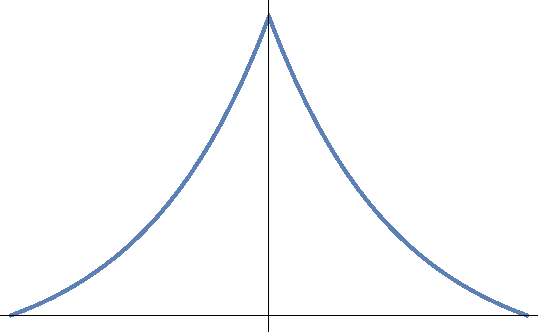
\includegraphics[width=0.45\textwidth]{Psi1.pdf}}
			            \subfigure[]{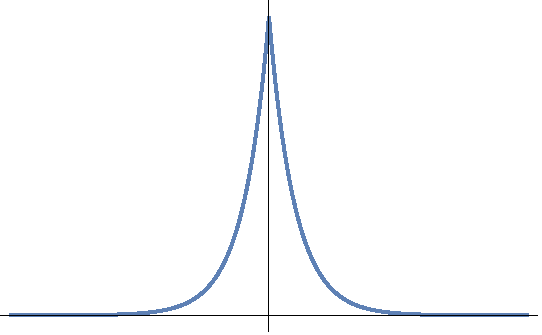
\includegraphics[width=0.45\textwidth]{Psi2.pdf}}
			            \caption{\(\Psi(x,0)\)}
			            \label{fig:subfigures}
		            \end{figure}
		            \begin{figure}[H]
			            \centering
			            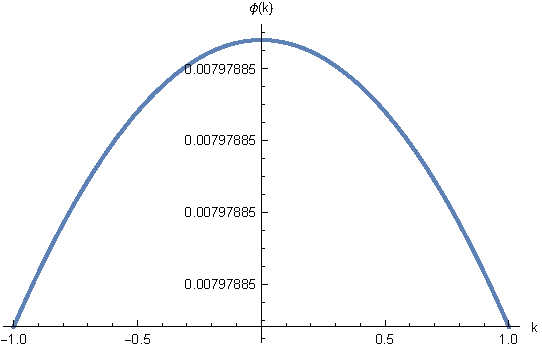
\includegraphics[width=0.5\textwidth]{phi.pdf}
			            \caption{\(\phi(k)\) when a = 10000}
		            \end{figure}
		      \item when a is very small, the graphs will be reverse from what we have when a is large.
	      \end{itemize}
\end{enumerate}

\subsection*{Problem 2.21}
\[\Psi(x,0) = A e^{-ax^2}\]
\begin{enumerate}[label=(\alph*)]
	\item Normalize the wave function:
	      \begin{align*}
		      1             & = \int_{-\infty}^{\infty} |\Psi(x,0)|^2 dx                               \\
		                    & = \int_{-\infty}^{\infty} |A e^{-ax^2}|^2 dx                             \\
		                    & = A^2 \int_{-\infty}^{\infty} e^{-2ax^2} dx  = A^2 \sqrt{\frac{\pi}{2a}} \\
		      \Rightarrow A & = \left(\frac{2a}{\pi}\right)^{\frac{1}{4}}                              \\
	      \end{align*}
	\item Find the wave function:
	      \begin{align*}
		      \phi(k)   & = \frac{1}{\sqrt{2 \pi}} \int_{-\infty}^{\infty} \Psi(x,0) e^{-ikx} dx                                                                                                      \\
		                & = \frac{1}{\sqrt{2 \pi}} \int_{-\infty}^{\infty} \left(\frac{2a}{\pi}\right)^{\frac{1}{4}} e^{-ax^2 -ikx}  dx                                                               \\
		                & = \frac{1}{\sqrt{2 \pi}} \left(\frac{2a}{\pi}\right)^\frac{1}{4} \int_{-\infty}^{\infty} e^{-ax^2 -ikx}  dx                                                                 \\
		                & = \frac{1}{\sqrt{2 \pi}} \left(\frac{2a}{\pi}\right)^\frac{1}{4} e^{-\frac{k^2}{4a}} \sqrt{\frac{\pi}{a}} = \frac{1}{(2a\pi)^\frac{1}{4}} e^{-\frac{k^2}{4a}}               \\
		      \Psi(x,t) & = \frac{1}{\sqrt{2\pi}} \int_{-\infty}^{\infty} \frac{1}{(2a\pi)^\frac{1}{4}} e^{-\frac{k^2}{4a}} e^{i(kx - \frac{\hbar k^2}{2m}t)} dk                                      \\
		                & = \frac{1}{\sqrt{2\pi}} \frac{1}{(2a\pi)^\frac{1}{4}} \int_{-\infty}^{\infty} e^{-\left(\frac{1}{4a} + \frac{i \hbar }{2m}t\right)k^2 + ikx} dk                             \\
		                & = \frac{1}{\sqrt{2\pi}} \frac{1}{(2a\pi)^\frac{1}{4}} e^{-\frac{x^2}{4\left(\frac{1}{4a}+ \frac{i \hbar}{2m }t\right)}} \sqrt{\frac{\pi}{\frac{1}{4a}+ \frac{i\hbar}{2m}t}} \\
		                & = \left(\frac{2a}{\pi}\right)^\frac{1}{4} \frac{1}{\gamma}e^{\frac{-ax^2}{\gamma^2}}, \quad \gamma = \sqrt{1 + \frac{2 i \hbar a t}{m}}
	      \end{align*}
	\item Find \(|\Psi(x,t)|^2\):
	      \[\omega = \sqrt{\frac{a}{\left[1+ \left(\frac{2 \hbar a t}{m}\right)^2\right]}}\]
	      \begin{align*}
		      |\Psi(x,t)|^2 & = \Psi^* \Psi                                                                                                                                                                                                       \\
		                    & = \left(\frac{2a}{\pi}\right)^\frac{1}{4} \frac{\left(e^{\frac{-ax^2}{\gamma^2}}\right)^*}{\gamma^*} \left(\frac{2a}{\pi}\right)^\frac{1}{4} \frac{e^{\frac{-ax^2}{\gamma^2}}}{\gamma}                              \\
		      \\
		                    & \text{instead of setting } \gamma = \sqrt{1 + \frac{2 i \hbar a t}{m}} \text{, we set } \gamma = \frac{2 \hbar a t}{m} \text{, then we have:}                                                                       \\
		                    & = \left(\frac{2a}{\pi}\right)^\frac{1}{2} \frac{\left(e^{-\frac{ax^2}{1+i \gamma}}\right)^*}{\left(\sqrt{1 + i \gamma}\right)^*} \frac{\left(e^{-\frac{ax^2}{1+i \gamma}}\right)}{\left(\sqrt{1 + i \gamma}\right)} \\
		                    & = \left(\frac{2a}{\pi}\right)^\frac{1}{2} \frac{\left(e^{-\frac{ax^2}{1-i \gamma}}\right)}{\left(\sqrt{1 - i \gamma}\right)} \frac{\left(e^{-\frac{ax^2}{1+i \gamma}}\right)}{\left(\sqrt{1 + i \gamma}\right)}     \\
		                    & = \left(\frac{2a}{\pi}\right)^\frac{1}{2} \frac{e^{-\frac{ax^2}{1-i \gamma}} e^{-\frac{ax^2}{1+i \gamma}}}{\sqrt{1 - i \gamma} \sqrt{1 + i \gamma}}                                                                 \\
		                    & = \left(\frac{2a}{\pi}\right)^\frac{1}{2} \frac{e^{-\frac{2ax^2}{1 + \gamma^2}}}{\sqrt{1 + \gamma^2}}                                                                                                               \\
	      \end{align*}
	      We can rewrite \(\omega = \sqrt{\frac{a}{\left(1+\gamma^2\right)}}\), then \(|\Psi(x,t)|^2\) can be written as:
	      \[\sqrt{\frac{2}{\pi}} \omega e^{-2 \omega^2 x^2}\]
	      For t = 0, we have:
	      \begin{figure}[H]
		      \centering
		      \subfigure[]{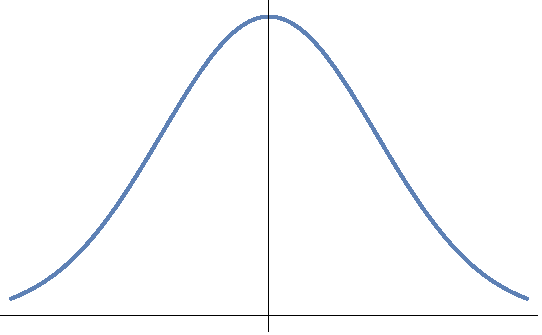
\includegraphics[width=0.45\textwidth]{psi^2.pdf}}
		      \caption{\(|\Psi(x,0)|^2\)}

	      \end{figure}
	      For t very large we have:
	      \begin{figure}[H]
		      \centering
		      \subfigure[]{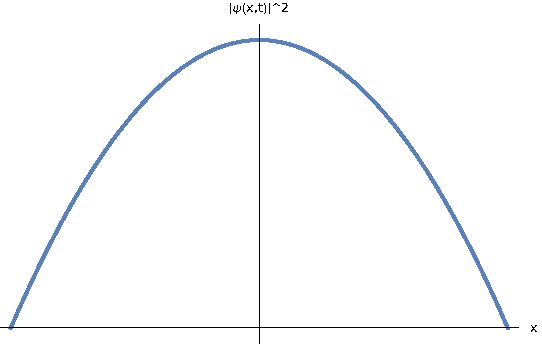
\includegraphics[width=0.45\textwidth]{psi^2.2.pdf}}
		      \caption{\(|\Psi(x,0)|^2, \quad t \rightarrow \infty\)}

	      \end{figure}
	\item Find \(\langle x \rangle, \langle p \rangle, \langle x^2 \rangle, \sigma_x, \sigma_p: \)
	\begin{align*}
		\langle x \rangle &= \int_{-\infty}^{\infty} x |\Psi(x,t)|^2 dx \\
		& = \int_{-\infty}^{\infty} x \sqrt{\frac{2}{\pi}} \omega e^{-2 \omega^2 x^2} dx \\
		&= \sqrt{\frac{2}{\pi}} \omega \int_{-\infty}^{\infty} x e^{-2 \omega^2 x^2} dx = 0 \quad \text{because }x e^{-2 \omega^2 x^2} \text{is an odd function}\\
		\langle p \rangle &= m \frac{d \langle x \rangle}{dt} = 0 \\
		\langle x^2 \rangle &= \int_{-\infty}^{\infty} x^2 |\Psi(x,t)|^2 dx \\
		& = \sqrt{\frac{2}{\pi}} \omega \int_{-\infty}^{\infty} x^2   e^{-2 \omega^2 x^2} dx \\
		&= \sqrt{\frac{2}{\pi}} \omega \frac{\sqrt{\pi}}{2(2 \omega^2)\sqrt{2 \omega^2}} = \frac{1}{4 \omega^2} \\
		\sigma_x &= \sqrt{\langle x^2 \rangle - \langle x \rangle^2} = \frac{1}{2 \omega} \\
		\sigma_p &= \sqrt{\langle p^2 \rangle - \langle p \rangle^2} = \sqrt{a} \hbar
	\end{align*}
	\item The uncertainty principle \(\sigma_x \sigma_p \geq \frac{\hbar}{2}\):
	\begin{align*}
		\sigma_x \sigma_p &= \frac{1}{2 \omega} \sqrt{a} \hbar = \frac{1}{2} \sqrt{\frac{1+\gamma^2}{a}} \hbar \sqrt{a} = \frac{\sqrt{1+\gamma^2}}{2} \hbar \geq \frac{\hbar}{2}
	\end{align*}
\end{enumerate}
\subsection*{Problem 2.22}
\[\int_{-3}^{1} (x^3 - 3x^2 + 2x - 1) \delta(x+2) dx\]
\[\int_{-\infty}^{\infty} f(x) \delta(x-a) dx = f(a) \]
\[\int_{-3}^{1} (x^3 - 3x^2 + 2x - 1) \delta(x+2) dx = (-2)^3 - 3(-2)^2 + 2(-2) - 1 = -8 - 12 - 4 - 1 = -25\]

\[\int_{0}^{\infty} \left[\cos(3x) + 2 \right]  \delta(x - \pi) dx = \cos(3 \pi) + 2 = -1\]

\[\int_{-1}^{1} \exp(|x| + 3) \delta(x-2) dx = 0\]

\subsection*{Problem 2.23}
\begin{enumerate}[label=(\alph*)]
	\item \(\delta(cx) = \frac{1}{|c|} \delta(x)\)
	      \[\int_{-\infty}^{\infty} f(x) \delta(cx) dx = \int_{-\infty}^{\infty} f(x) \frac{1}{|c|} \delta(x) dx = \frac{1}{|c|} f(0), \quad c \in \mathbb{R}\]
	\item \(\frac{\partial \theta}{dx} = \delta(x)\)
	      \[\int_{-\infty}^{\infty} f(x) \frac{\partial \theta}{dx} dx = \int_{-\infty}^{\infty} f(x) \delta(x) dx = f(0)\]
\end{enumerate}

\subsection*{Problem 2.26}
\[\delta(x) = f(x)  = \frac{1}{\sqrt{2 \pi}} \int_{-\infty}^{\infty} F(k) e^{i k x} dk  \]
\[F(k)  = \frac{1}{\sqrt{2 \pi}} \int_{-\infty}^{\infty} f(x) e^{-i k x} dx = \frac{1}{\sqrt{2 \pi}} \int_{-\infty}^{\infty} \delta (x) e^{-i k x} dx = \frac{1}{\sqrt{2\pi}}\]
Substitute back to the first equation, we have:
\[\delta(x) = \frac{1}{\sqrt{2 \pi}} \int_{-\infty}^{\infty} \frac{1}{\sqrt{2\pi}} e^{i k x} dk = \frac{1}{2 \pi} \int_{-\infty}^{\infty} e^{i k x} dk\]

\end{document}